The Silicon Photomultiplier (SiPM) are a kind of photosensor, based on semiconductor materials, developed in recent years. They are replacing progresively conventional PMTs in many experiments and applications. They archieve outstading photon-counting capabilities with high gain and high photodetection efficiency comparing to PMT. They have conveninent characteristics as insensitiveness to magnetic fields, low operating voltage and compactness.

SiPM are based on p-n junctions, made with special techniques to archieve a good contact between both surfaces.

The voltage at which the SiPM starts operating in geiger mode is called the breakdown voltage, $ V_ {BR} $. At a lower voltage it works in proportional mode. The measurement of the breakdown voltage is one of the most important parametes to characterize the SiPM and its experimental measurements is described in section \ref{sec:CharacterizationSiPM}.

The SiPM is formed by a matrix of APDs which are photodiodes operating in Geiger mode. A scheme of an APD is shown in Figure \ref{fig:SchemeAPD}. It has p+ and a n+ layers. 

\begin{figure}[htbp]
\centering
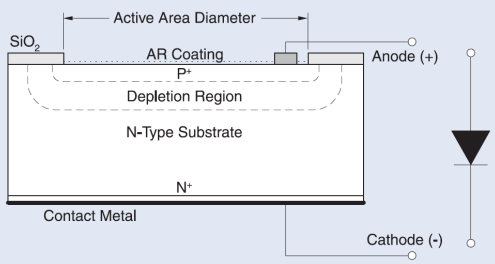
\includegraphics[scale=0.6]{3DesignPrinciples/32Tritium_detector/APD_scheme.png}
\caption{Scheme of a APD and electrical symbol used.\label{fig:SchemeAPD}~\cite{OSI}}
\end{figure}
 
These APDs, called pixels when they are part of a SiPM, are connected in parallel and the sum of all of them is read. The output signal of the pixels are quite similar regardless of the energy deposited, with some difference because of the uncertainty due to the SiPM manufacturing process and the statistical nature of the detection process. The energy deposited in each APD is not known but, as all SiPM pixels are read at the same time, the charge of the output signal when n photons are simultaneously detected is n times the charge of a single photon, as can be seen in Figure \ref{fig:PulsesOfSiPM}. Due to this property, after a correct calibration of SiPMs the number of detected photons we have detected is linearly related to the output signal. 

As the number of scintillating photons is proportional to the deposited energy, the linearity of its output signal and the deposited energy is recovered.

\begin{figure}[htbp]
\centering
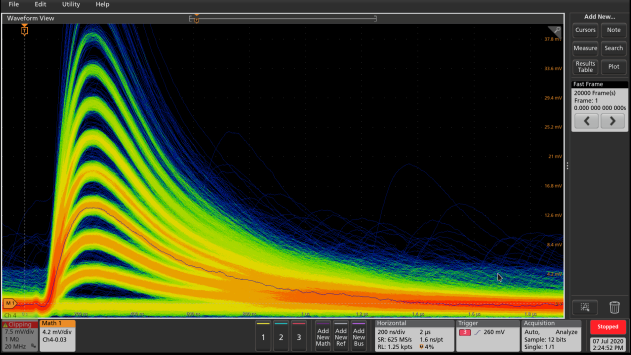
\includegraphics[scale=0.6]{3DesignPrinciples/32Tritium_detector/Several_SiPM_pulses.png}
\caption{Using persistence on the oscilloscope to show several pulses with different heights. Each height associated with a different number of  SiPM pixels lit at the same time.\label{fig:PulsesOfSiPM}}
\end{figure}

On top of that, these pixels need to be so small\footnote{Pixel sizes for commercial SiPMs are $50$ or $75\mu\meter$ \cite{DataSheetHammamatsu_1_SiPM_50}, \cite{DataSheetHammamatsu_1_SiPM_75}} that, if the photon density to be detected is low enough, we only detect one photon in each pixel. If it doesn't happen, we will detect two or more photons with the same pixel but the output signal will be the same as one detected photon, so we will have a loss of linearity of our output signal. This effect is known as saturation and it is important to know the photon density at which it happens for our SiPMs. %The experimental measurements of this effect, which have been done for our SiPMs, is shown in section \ref{sec:CharacterizationSiPM}. 

Each of these pixels has a quenching resistance\footnote{The tipical valuer of this quenching resistance for commercial SiPMs is around $500~\kilo\Omega$} in series that is used to stop the current produced when this pixel has detected a particle. It is used for limit the current drawn by the diode during breakdown and reduce the reverse voltage seen by the diode to one below the breakdown voltage. After that, the voltage seen by the diode is reset to the bias voltage and this pixel is ready to detect a new photon again. In Figure \ref{fig:ChenchingResistance} (left) a diagram of these chenching resistances and APDs in a SiPM and (right) how it works is shown respectively.

\begin{figure}
\centering
    \begin{subfigure}[b]{0.45\textwidth}
    \centering
    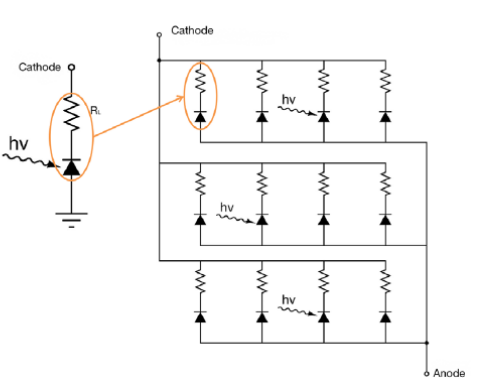
\includegraphics[width=\textwidth]{3DesignPrinciples/32Tritium_detector/Quenching_resistence_of_a_SiPM_scheme.png}  
    \caption{Photon Detection Efficiency, PDE.\label{subfig:ElectricModelSiPM}}
    \end{subfigure}
    \hfill
    \begin{subfigure}[b]{0.45\textwidth}
    \centering
    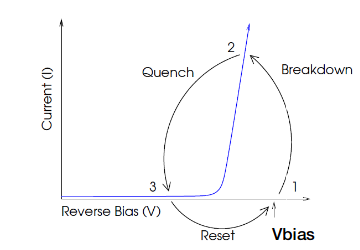
\includegraphics[width=\textwidth]{3DesignPrinciples/32Tritium_detector/How_a_quenching_resistence_in_a_SiPM_works.png}  
    \caption{Output current of a SiPM.\label{subfig:HowSiPMworks}}
    \end{subfigure}
 \caption{(Left) Electronic scheme of a SiPM and (right) output current of a SiPM as a function of the reverse voltage. It show that the quenching mechanism is essential for working with SiPMs~\cite{DataSheetSensL}.}
 \label{fig:ChenchingResistance}
\end{figure}

In this simple electrical scheme we can see that all pixels have a common cathode and anode which means that, as we said before, they are at the same bias voltage and the output is the sum of all of them.

We have a lot of names to refer to these photosensors such as SiPMs, MPPCs, G-APDs, SSPMs, MRS-ADPs or AMPDs. The candidate for TRITIUM project is S13360-6075 from Hamamatsu photonics \cite{DataSheetHammamatsu_1_SiPM_75} because its characteristics are the ones that best fit our objectives since this model has super low afterpulses, crosstalk and dark counts than other SiPM models from Hamamatsu. Its characteristics and properties are shown in Table \ref{tab:PropertiesOfSiPM75}. 

\begin{table}[htbp]
%%\centering.
\begin{center}
\begin{tabular}{|c|c|}
\hline
Parameter & Numerical value \\
\hline \hline \hline
Serie & $S13360$ \\ \hline
Model & $6075$ \\ \hline
Pixel Pitch ($\mu\meter$) & $75$ \\ \hline
Effective photosensitive area ($\mm^2$) & $6.0 \times 6.0$ \\ \hline
Number of pixels & $6400$ \\ \hline
Fill factor & $82\%$ \\ \hline
Refractive index of windows material & $1.55$ \\ \hline
Operating temperature range ($\degree C$)& $[-20,60]$ \\ \hline
Spectral response range, $\lambda$ ($\nano\meter$) & $[320, 900]$ \\ \hline
Peak sensitivity wavelength, $\lambda_p$ ($\nano\meter$) & $450$ \\ \hline
PhotoDetection Efficiency, PDE, $\lambda=\lambda_p$ ($\%$) & $50$ \\ \hline
Dark counts, Typical/Maximum (kcps) & $2000/6000$ \\ \hline
Terminal capacitance, $C_t$ ($\pico\farad$) & $1280$ \\ \hline
Gain, M, & $4 \cdot{} 10^6$ \\ \hline
Breakdown Voltage, $V_{BR}$ ($\volt$) & $53$ \\ \hline
Cross talk probability($\%$) & $7$ \\ \hline
Temperature coefficient $\Delta TV_{op}$ (m$\volt/\degree C$) & $54$ \\ \hline
\end{tabular}
\caption{Characteristics of SiPM S13360-6075 from Hamamatsu Photonics \cite{DataSheetHammamatsu_1_SiPM_75}.}
\label{tab:PropertiesOfSiPM75}
\end{center}
\end{table}

These values, provided by Hamamatsu photonics, are only approximate for a given element. Therefore, these parameters must be measured experimentally for each SiPM because they can vary significatively even for SiPMs of the same model. The most important characteristics for the TRITIUM project are experimentaly measured and given in section \ref{sec:CharacterizationSiPM}. 

Although TRITIUM detector uses whole SiPM matrices, the caracterizations has been carried out at the level of a single SiPM (same model) to learn about the values of the SiPM parameters and to test the gain control method.
 
The matrices selected are of the model "S13361-6050" from Hamamatsu, which consists of a $4\times 4$ SiPM matrix where the active area of each SiPM is $6\times 6~\mm$ \cite{DataSheetHammamatsu_array_SiPM_6050} or the model "S13361-3050" from Hamamatsu, which consists of a $8\times 8$ SiPM where the active area is $3\times 3~\mm$ \cite{DataSheetHammamatsu_array_SiPM_3050}. They are commercial matrices from Hamamatsu and the total active area that is covered is the same for both models, $24\times 24~\mm$ and it is approximatelly the same as the active area covered with the PMTs employed, described in the previous section. These matrices have a common bias voltage and ground for all SiPMs but a different output signal for each SiPM. 

%We hope to obtain better results with the 4x4 matrix for theoretical reasons which we will see in section \ref{sec:CharacterizationSiPM} like larger PDE, mainly due to a larger active area but it is something that we will have to verify with experimental measurements.